\documentclass[conference]{IEEEtran}
\usepackage{booktabs}
\usepackage{amsmath,amssymb}
\usepackage{graphicx}
\usepackage{url}
\usepackage[hidelinks]{hyperref}

\begin{document}

\title{Text Chunking Strategies for Retrieval-Augmented Generation over University Course Policies}

\author{\IEEEauthorblockN{Juncheng Qian}
\IEEEauthorblockA{CPS5801, WKU\\
Email: \texttt{qianjun@kean.edu}}}

\maketitle

\begin{abstract}
Retrieval-augmented generation (RAG) over university course policies must return a complete policy clause, including its exception, rather than a passage that merely overlaps the answer. We study how text chunking affects this evidence-complete retrieval under a controlled protocol: one frozen corpus, one frozen bi-encoder, one fixed set of 17 chunking configurations, and one shared frozen cross-encoder reranker checkpoint. Gold evidence is annotated on the original documents, independent of any chunking, and completeness is scored on the union of the retrieved character intervals. Across the 17 configurations on the first test split, mean Complete@10 increased from 0.358 under C1 (dense top-50) to 0.405 under C3 (top-50 with reranking); the paired C3$-$C1 difference was $+0.047$ (95\% CI $[-0.005,+0.095]$) and is not significant. On a pre-registered supplementary set of 45 single-clause questions in 45 groups, the structural-minus-semantic difference on C1 was $+0.800$ (95\% CI $[0.666,+0.911]$), and C3$-$C1 was $+0.052$ (95\% CI $[0.020,+0.089]$). The results support a corpus- and protocol-scoped conclusion: the tested structure-aware configurations retrieve complete evidence more often than the tested sentence-level semantic configurations, while the reranking effect was not supported as a non-zero effect on the first test split and was positive but imprecisely estimated on the supplementary set.
\end{abstract}

\begin{IEEEkeywords}
retrieval-augmented generation, chunking, evidence completeness, passage retrieval, reranking
\end{IEEEkeywords}

\section{Introduction}
University course policies are rule-dense: a correct answer often depends on a general rule and on an exception that appears in another sentence or section. A RAG system that retrieves only the rule can look relevant while still being insufficient for a correct answer. Conventional any-hit and first-relevant-rank metrics do not require retrieval of every evidence item needed for an answer.

We address two research questions:
\begin{itemize}
\item \textbf{RQ1:} How do chunking strategies affect evidence-complete retrieval over course-policy documents?
\item \textbf{RQ2:} Under a controlled candidate-pool design, does cross-encoder reranking improve evidence completeness or alter the ranking of chunking strategies?
\end{itemize} We build a frozen corpus of 36 university policy documents, annotate gold evidence on the original text, and compare 17 chunking configurations from four families under a frozen encoder and the same indexing and search procedure, with a separate index for each configuration. A 2$\times$2 design separates candidate-pool size from reranking, and a second, pre-registered question set checks the main family difference on unseen questions.

Consider a late-submission policy with a general rule (a deduction per late day) and an exception (an approved extension is not late). A retriever that returns only the rule has a passage that fully covers one required gold clause and therefore a non-zero Hit@$k$, yet it cannot support the correct answer for a question that asks about both cases. This example, which is fictitious but representative of the corpus, motivates scoring the union of retrieved evidence rather than a single passage.

Our contributions are:
\begin{itemize}
\item An evaluation design in which gold evidence is annotated independently of chunking, retrieved evidence is merged by character-interval union, and evidence recall and Complete@$k$ are reported separately from MRR; partial coverage is defined and released per question.
\item A controlled comparison of 17 chunking configurations across four tracks, separating candidate-pool expansion from reranking.
\item An empirical study of the structural-versus-semantic difference on this corpus and protocol, including a pre-registered supplementary check on a single-clause question set.
\end{itemize}

We do not claim that union-based completeness is a new metric, nor that the findings generalise beyond this corpus and protocol.

\section{Related Work}
\subsection{Chunking for retrieval-augmented generation}
Chunking decisions determine what a retriever can return. Recent studies compare fixed, recursive, semantic and structure-aware splitting on institutional, regulatory and clinical documents \cite{fadillah2024chunking,gomez2025chunking,khalib2026chunking}. Khalib et al.\ compare chunking strategies over structured institutional documents and evaluate retrieval hits, answer quality and table completeness \cite{khalib2026chunking}. Their setting is the closest to ours, but it does not ask whether the retrieved passages jointly provide all evidence required by a multi-part policy question.

\subsection{Semantic and structure-aware splitting}
Semantic chunking merges sentences according to embedding similarity \cite{kiss2025maxmin,moreno2026growing}, while paragraph- and heading-based methods follow document structure \cite{mazzitelli2025paragraph}. Moreno-Cediel et al.\ propose a growing-window semantic strategy for weak semantic boundaries \cite{moreno2026growing}. These studies motivate our hypothesis that sentence-level semantic boundaries can fragment a policy clause, but they evaluate retrieval with passage-level relevance rather than evidence completeness.

\subsection{Evidence completeness and document QA}
Benchmarks for document analysis and table reasoning expose cases where several pieces of evidence are needed \cite{hui2024uda,yu2025tablerag}, and RAG evaluation frameworks score answer faithfulness and context quality \cite{es2024ragas,wang2024bestpractices}. Our metric is narrower: it asks whether the union of retrieved intervals covers every annotated evidence span, and it deliberately keeps MRR as a separate single-chunk ordering measure.

\textbf{Relation to the two closest studies.}
Khalib et al.\ compare chunking strategies over structured institutional documents and evaluate retrieval hits, answer quality and table completeness \cite{khalib2026chunking}; their task and document type are close to ours, but their unit of evaluation is a retrieved passage or table, not the joint coverage of several annotated clauses. Moreno-Cediel et al.\ study semantic boundaries and propose a growing-window strategy \cite{moreno2026growing}; their focus is boundary quality in encyclopaedic text, not whether a policy rule and its exception are retrieved together. Our study keeps both concerns in one design: the chunking families include the semantic alternative, the documents are institutional policy text, and the outcome is complete gold evidence, which neither study measures directly.

\subsection{Retrieval and reranking foundations}
Dense retrieval represents questions and passages in a shared embedding space and retrieves the nearest passages \cite{karpukhin2020dpr}; RAG conditions a generator on retrieved passages \cite{lewis2020rag}. Cross-encoder rerankers score query--passage pairs jointly and are typically applied to a small candidate pool \cite{nogueira2019passage}, while bi-encoder sentence representations enable efficient first-stage search \cite{reimers2019sbert}. Pretrained sequence-to-sequence rankers also score query--document pairs jointly and improve document ranking \cite{nogueira2020document}. Benchmarks such as BEIR show that retrieval difficulty varies sharply across domains and that no single retriever dominates \cite{thakur2021beir}. These components motivate our frozen encoder, exact inner-product index and single shared reranker, which hold the retrieval stack constant while chunking varies.

\subsection{Research gap}
The literature compares chunking families but rarely holds the encoder, indexing/search procedure, questions and top-$k$ fixed while measuring complete evidence retrieval on policy text. This study fills that gap with a controlled comparison and a pre-registered second question set, while restricting its claims to the tested corpus and protocol.

\section{Methodology}
\subsection{Corpus and evidence annotation}
The corpus contains 36 publicly accessible university policy documents (14 course, 9 faculty, 13 institution; 12 institutions; 1,988 clauses). Each document is stored twice: a character-faithful evidence layer, on which all gold spans are defined, and a normalised retrieval layer with a character map back to the evidence layer. Gold evidence is annotated as character intervals $(d,a,b)$ on the evidence layer; it is never defined on chunks, so every configuration is scored against the same reference.

\begin{table}[t]
\centering
\caption{Corpus and question sets. Evidence groups are disjoint across splits.}
\label{tab:data}
\small
\resizebox{\columnwidth}{!}{%
\begin{tabular}{lr}
\toprule
item & value\\
\midrule
documents & 36 (14/9/13 course/faculty/institution)\\
institutions & 12\\
clauses & 1,988\\
first set questions & 172 (112 dev / 60 test)\\
first set groups & 59 test groups\\
second set questions & 45 (45 groups; single-clause)\\
\bottomrule
\end{tabular}}
\end{table}

\textbf{Annotation and quality control.}
Each question was written against a frozen evidence bundle, and every cited clause was checked against the evidence layer before the split was locked. The first set was drafted by the AI and reviewed question by question by us (23 defects corrected); test2 was drafted by the AI; before the lock, an AI self-audit recorded two answer corrections (T2Q003, T2Q021). After our review of the 45 questions was complete, we jointly reviewed them with the AI (attestation dated 2026-11-21); no locked question was changed. A question's evidence is stored as one or more alternative sufficient sets, so a system is not penalised for finding a different valid combination of clauses. A second independent human annotator was not available, so we did not estimate inter-annotator agreement. To reduce annotation risk, we checked every cited clause against the character-faithful evidence layer, used fixed evidence-set rules, and preserved alternative sufficient evidence sets. Boundary decisions were not independently replicated, which remains a limitation.

\textbf{Composition and split discipline.}
The 36 documents span course syllabi, faculty handbooks and institution-wide regulations; the largest single source is Glasgow, which supplies roughly one third of the clauses, and the remaining documents come from eleven other institutions. Questions were split by group (same wording family and inference shape). A separate evidence-overlap audit verified that no gold clause is shared between development and test; it reports zero crossing clauses. test2 was drawn only from clauses unused by any existing question, and its lock check reported no leakage. The first set deliberately mixes single-clause, rule-and-exception and cross-clause questions; the second set is restricted to single-clause questions by design. This difference is central to how the two sets may be interpreted and is revisited in the limitations.

\subsection{Chunking configurations}
We evaluate 17 configurations from four families (Table~\ref{tab:configs}). Fixed-length windows use four target sizes and three overlaps; paragraph and heading configurations merge corpus units at the corresponding structural boundary; semantic configurations merge adjacent sentences while their embedding cosine similarity exceeds a threshold. Any over-long unit is split further at sentence and then token boundaries. Two limits are distinct: the pipeline caps a chunk at 512 tokens, and the encoder itself has a 512-token maximum input.

\begin{table}[t]
\centering
\caption{The 17 chunking configurations. Fixed windows contribute 12 configurations (4 sizes $\times$ 3 overlaps; all overlaps are smaller than every size).}
\label{tab:configs}
\small
\resizebox{\columnwidth}{!}{%
\begin{tabular}{llc}
\toprule
family & configuration & count\\
\midrule
fixed & size $\in\{128,256,384,512\}$ $\times$ overlap $\in\{0,32,64\}$ & 12\\
paragraph & merge at paragraph boundaries & 1\\
heading & merge at heading boundaries & 1\\
semantic & cosine threshold $\in\{0.70,0.75,0.80\}$ & 3\\
\midrule
total & & \textbf{17}\\
\bottomrule
\end{tabular}}
\end{table}

The configuration set is a family comparison, not a search for the best single method. Fixed windows give controlled size and overlap baselines; paragraph and heading preserve natural document boundaries; the three semantic thresholds (0.70, 0.75, 0.80) are a sensitivity range for similarity-based merging, not dev-selected optima. All configurations share the same corpus, evidence layer, 512-token chunk cap, frozen encoder, FAISS search procedure, candidate-pool sizes, questions and metrics. These controls make the retrieval treatment comparable, but they do not equalize chunk-length distributions, boundary placement, redundancy, or the number of chunks that fit a budget; chunk length remains part of the practical effect of a strategy.

\subsection{Metrics}
Let $R_k$ be the first $k$ retrieved chunks in rank order. For a document $d$, let $U_d(R_k)$ be the union of the evidence intervals of those chunks that belong to $d$; overlapping chunks therefore do not double-count evidence.

For a question $q$ with a family of alternative sufficient evidence sets $\mathcal{S}_q$, each set $S=\{(d,a,b)\}$, a span is covered when $[a,b)\subseteq U_d(R_k)$. In this release each annotated clause has exactly one span, so $|S|$ is the number of clauses in the set and Recall@$k$ below is clause-level. The tuple $(d,a,b)$ denotes the half-open interval $[a,b)$. All intervals are half-open character ranges $[a,b)$, matching Python slicing. Formally, with $R_k$ the first $k$ chunks,
\begin{equation}
U_d(R_k)=\bigcup_{c\in R_k,\,c.d=d}\bigcup_{[s,e)\in c.\mathrm{ev}}[s,e),
\end{equation}
so only character intervals count, chunk identifiers do not. A sufficient set is covered when every one of its spans is contained in the corresponding union.

\textbf{Hit@$k$} is 1 when the union of the first $k$ chunks fully covers at least one required gold clause (from any sufficient set), and 0 otherwise.

\textbf{Evidence recall@$k$} is the maximum, over sufficient sets $S$, of the fraction of clauses in $S$ that are fully covered:
\begin{equation}
\mathrm{Recall@}k=\max_{S\in\mathcal{S}_q}\frac{1}{|S|}\sum_{(d,a,b)\in S}\mathbf{1}\{[a,b)\subseteq U_d(R_k)\}.
\end{equation}

\textbf{Complete@$k$} is 1 when some sufficient set is fully covered by the union, and 0 otherwise.

\textbf{Partial coverage} is the mean, over all spans of all sufficient sets, of the covered character fraction $|[a,b)\cap U_d(R_k)|/|[a,b)|$; it is reported separately because it is not the same as the per-clause recall above.

\textbf{MRR} uses the first single chunk whose evidence intervals fully cover any required clause; partial intersection does not count. Complete and Hit are cumulative-set metrics, whereas MRR is a single-position metric, and the paper keeps them separate.

\subsection{Aggregation}
Metrics are computed per question. Questions are averaged equally within a question group; configurations are then averaged equally within the group (17 overall, or the family's configurations for family results). Uncertainty is obtained by a paired bootstrap over groups ($B=2000$, seed 20261013) with shared resampling indices, and percentile 2.5/97.5 intervals are reported. Questions are equally weighted within a group, groups are equally weighted in the bootstrap, and configurations are equally weighted; this is not equal weighting over all questions globally. The secondary endpoint C3$-$C1 averages the same 17 configurations in each track.

\subsection{Reranker}
The reranker is \texttt{BAAI/bge-reranker-base} \cite{bge_reranker}, an XLM-RoBERTa-base cross-encoder (12 layers, hidden size 768), trained with a binary cross-entropy objective with logits on query--chunk pairs. Ten of the twelve encoder layers are frozen, leaving 85.6M trainable parameters, and the model is trained with Adafactor for at most three epochs with early stopping (patience 1). Pairs are built from the top-50 candidate pools of the 17 configurations; each positive is paired with four hard negatives, and partial-overlap pairs are excluded from the loss.

\textbf{Implementation details.}
The encoder is \texttt{bge-small-en-v1.5}: 384-dimensional CLS-pooled embeddings, L2-normalised, with no instruction prefix added to queries. The index is FAISS \texttt{IndexFlatIP} (exact inner-product search), one index per configuration. The reranker uses the checkpoint tokenizer and a manual pair construction \texttt{[CLS] query [SEP] chunk [SEP]}: the query is truncated to 128 content tokens (special tokens excluded) and the chunk to $512-\mathrm{len}(\mathrm{query})-3$ content tokens, leaving room for exactly three special tokens. No second max-length truncation is applied. The XLM-R tokenizer's default pair API would reserve four special tokens, so the subtraction is specific to this construction. Token-budget accounting uses the encoder tokenizer, counts content tokens only (\texttt{add\_special\_tokens=False}), and admits chunks from the top-50 candidate pool in rank order. The learning-rate grid was $\{10^{-5},2\cdot10^{-5}\}$ with four negatives per positive.

\section{Experimental Setup}
\subsection{Splits and question sets}
The first set contains 172 questions (112 development, 60 test; 59 test groups) and includes single-clause, rule-and-exception and cross-clause evidence. The development split is group-disjoint: 89 training and 22 validation questions in 85 and 21 groups. One development question (Q0141) had no positive pair and was dropped, so 111 of the 112 development questions enter the reranker split (200 candidate rows dropped); these are the post-drop counts. The test split had been used once as a pilot before the reranker stage, so its results are exploratory re-evaluations of a seen split, not a pristine holdout.

The second set (test2) contains 45 questions in 45 groups and only single-clause questions. Its design was locked on 2026-11-13 (01:56) and evaluated once (02:01); answer revisions and composition amendments were recorded before evaluation (01:45). The composition is integrity-heavy (25/45), Glasgow contributes 15/45 (33\%), and all questions are single-clause. A joint author--AI review attestation is dated 2026-11-21, after the evaluation; no locked question was changed. The set supports family comparisons and complete-gold-evidence retrieval for single-clause questions, but it cannot directly validate multi-clause completeness.

\subsection{Tracks and baselines}
The four tracks are: main (dense top-10), C1 (dense top-50), C2 (top-10 with reranking) and C3 (top-50 with reranking). C1$-$main and C2$-$main are arithmetic identities for set-level metrics and are asserted to be zero rather than tested; the informative contrast is C3$-$C1. Baselines are the 17 chunking configurations under the same frozen encoder and indexing/search procedure, with one index per configuration.

\textbf{Comparability controls.} Only chunking changes: all configurations use the same corpus and gold evidence, the same frozen encoder, the same FAISS indexing/search procedure with one index per configuration, the same top-10/top-50 pools and reranker, and the same Complete/Recall/Hit/MRR definitions. Because fixed top-$k$ exposes different amounts of text, we add matched token budgets (512/1024/2048); complete chunks are admitted in rank order, the next over-budget chunk stops admission without truncation or skipping, and overlap is charged at its actual token count. These controls make the protocol comparable, but they do not make the resulting chunk distributions identical: chunk length, boundary placement, redundancy, and the number of chunks within a budget remain part of the practical effect.

\subsection{Training and model selection}
Table~\ref{tab:training} summarises the training settings. Within a run, the best epoch is chosen by macro reranked Complete@10 over the 17 configurations on the top-50 validation pool; a strictly larger value replaces the current best, so ties keep the earlier epoch. Early stopping uses the same metric with patience 1. Across runs, the same metric is used first, followed by macro MRR, macro Recall@10, a smaller learning rate and fewer negatives. The selected canonical checkpoint is the 10-layer-frozen model (lr $10^{-5}$, seed 20261027, validation Complete@10 0.3877). Compatibility runs (T06 full fine-tuning and the T07 learning-rate grid) are reported in \texttt{models/reranker/COMPAT.json} for reproducibility context; they are not part of the main experimental comparison or checkpoint selection.

\begin{table}[t]
\centering
\caption{Training settings. T06 and T07 are compatibility experiments, not the paper's checkpoint.}
\label{tab:training}
\small
\resizebox{\columnwidth}{!}{%
\begin{tabular}{lccc}
\toprule
item & partial (main) & T06 full & T07 grid\\
\midrule
frozen encoder layers & 10/12 & 0 & 10/12\\
optimizer & Adafactor & AdamW & Adafactor\\
learning rate & $10^{-5}$ & $10^{-5}$ & $\{10^{-5},2\cdot10^{-5}\}$\\
negatives/positive & 4 & 4 & 4\\
batch $\times$ accum & $8\times2$ & $32\times1$ & $8\times2$\\
epochs / patience & $\le3$ / 1 & $\le3$ / 1 & $\le3$ / 1\\
train/val groups & 85/21 & 85/21 & 85/21\\
seed & 20261027 & 20261027 & 20261027/47/57\\
role & \textbf{main} & compatibility & compatibility\\
\bottomrule
\end{tabular}}
\end{table}

\subsection{Statistics}
For the first test split, Holm correction is applied over $\{$C3$-$C1, C3$-$C2$\}$ for Complete@10, with ordering metrics corrected separately by family; we report effect sizes, 95\% confidence intervals and adjusted $p$-values. For test2, the pre-registered decision uses fixed-sequence gatekeeping: the primary endpoint is structural (heading and paragraph) minus semantic (thresholds 0.70/0.75/0.80) on C1, and it is confirmed only when the 95\% CI lower bound exceeds 0.30. Only then is the secondary endpoint C3$-$C1 interpreted; a positive gain is supported when its CI lower bound exceeds 0. Corrected p-values start from a two-sided paired bootstrap over group-level deltas, $p=2\min(P(\delta\le0),P(\delta\ge0))$ with $B=2000$ shared resamples and a floor of $1/B$; Holm is applied afterwards within the stated families. A reported Holm-adjusted $p=0.004$ for C3$-$C1 is supplementary and is not the pre-registered decision rule.

\textbf{Statistical power.}
The test2 design has limited power for a pre-specified small effect: with 45 groups, the minimum detectable effect for the secondary endpoint is about 0.079, with power 0.384 at 0.047 and 0.966 at 0.107; the primary endpoint's minimum detectable effect is about 0.184. The minimum detectable effect is defined at 80\% power and a two-sided 5\% level ($z_{0.975}+z_{0.80}$); these are design calculations, not a reinterpretation of the observed interval. The observed secondary interval excludes zero, so the data support a positive direction; the width of that interval, not the power calculation alone, is why the magnitude remains imprecise.

\subsection{Hardware, software and reproducibility}
Canonical results were produced on an NVIDIA RTX 3060 Laptop (6 GB); the A5000 (24 GB) was used for the T06 and T07 compatibility experiments and for the single test2 run. The artifact map records the test run on the RTX 3060 and test2/T06/T07 on the A5000; test and test2 use the same FROZEN checkpoint, while T06/T07 are separate compatibility runs and do not enter the main results. Software included PyTorch 2.6.0 with CUDA 12.4 and the Hugging Face \texttt{bge-small-en-v1.5} encoder \cite{bge_small}. The code, frozen corpus snapshot, official indexes, and checkpoint (with the matching config and tokenizer files) are released at \url{https://github.com/Xiaocao21/course-policy-rag/releases/tag/v0.1.5-repro}. The statistical recomputation reproduces both splits' \texttt{stats.json} with zero field differences, and the test2 retrieval replay reproduces 3,060 row-level comparisons (4 tracks $\times$ 17 configurations $\times$ 45 questions) with per-question values identical and official hashes unchanged; the evaluation environment is only partially recorded, so this is row-level agreement rather than proof that every historical detail matched.

\textbf{Artifact map.}
Every reported cell is mapped to a split, track, configuration, metric and source file in the released artifact map, and the flat result tables are generated from the same JSON files that feed the statistics. The frozen corpus snapshot, the official FAISS indexes and the checkpoint are separate release assets; the snapshot is needed because a fresh crawl no longer reproduces the original bytes. The official indexes are used for byte-identical replay of the archived run: rebuilding them produces different serialized bytes, so the hash-based pre-registration check would reject the rebuilt files. This is an archival-replay requirement, not evidence that retrieval behaviour differs. This separation lets a reader verify the statistics from committed files alone, or replay retrieval with the published assets, without conflating the two levels.

\section{Results}
\textbf{Main findings.} Three results organize this section. First, heading and paragraph chunking achieved the highest evidence completeness under both top-$k$ and matched token budgets. Second, the first test split did not provide statistically significant evidence of a non-zero reranking effect. Third, test2 showed a large structural--semantic gap and a positive reranking contrast, but its single-clause composition limits the conclusion.

Table~\ref{tab:test} reports the four tracks on the first test split. The three tracks scored on their first ten items (main, C1, C2) have identical set-level metrics, as expected: enlarging the dense pool to 50 does not change the top-10 set, and reranking the top-10 does not change set membership. C3 reaches Complete@10 0.405 [0.347, 0.464] against 0.358 [0.299, 0.418] for C1, a difference of $+0.047$ [$-0.005,+0.095$] (Holm-adjusted $p=0.150$). The gain is therefore not significant on this split. MRR is computed over each track's full candidate depth rather than a common MRR@10, so the main-to-C1 increase partly reflects the deeper pool.

\begin{table}[t]
\centering
\caption{First test split (60 questions, 59 groups). Complete@10 with group-bootstrap 95\% CI. MRR is evaluated over each track's candidate depth (10 for main/C2, 50 for C1/C3).}
\label{tab:test}
\small
\begin{tabular}{lcccc}
\toprule
track & pool & rerank & Complete@10 [95\% CI] & MRR\\
\midrule
main & 10 & no & 0.358 [0.299, 0.418] & 0.276\\
C1 & 50 & no & 0.358 [0.299, 0.418] & 0.282\\
C2 & 10 & yes & 0.358 [0.299, 0.418] & 0.312\\
C3 & 50 & yes & \textbf{0.405} [0.347, 0.464] & \textbf{0.322}\\
\bottomrule
\end{tabular}
\end{table}


\begin{figure}[t]
\centering
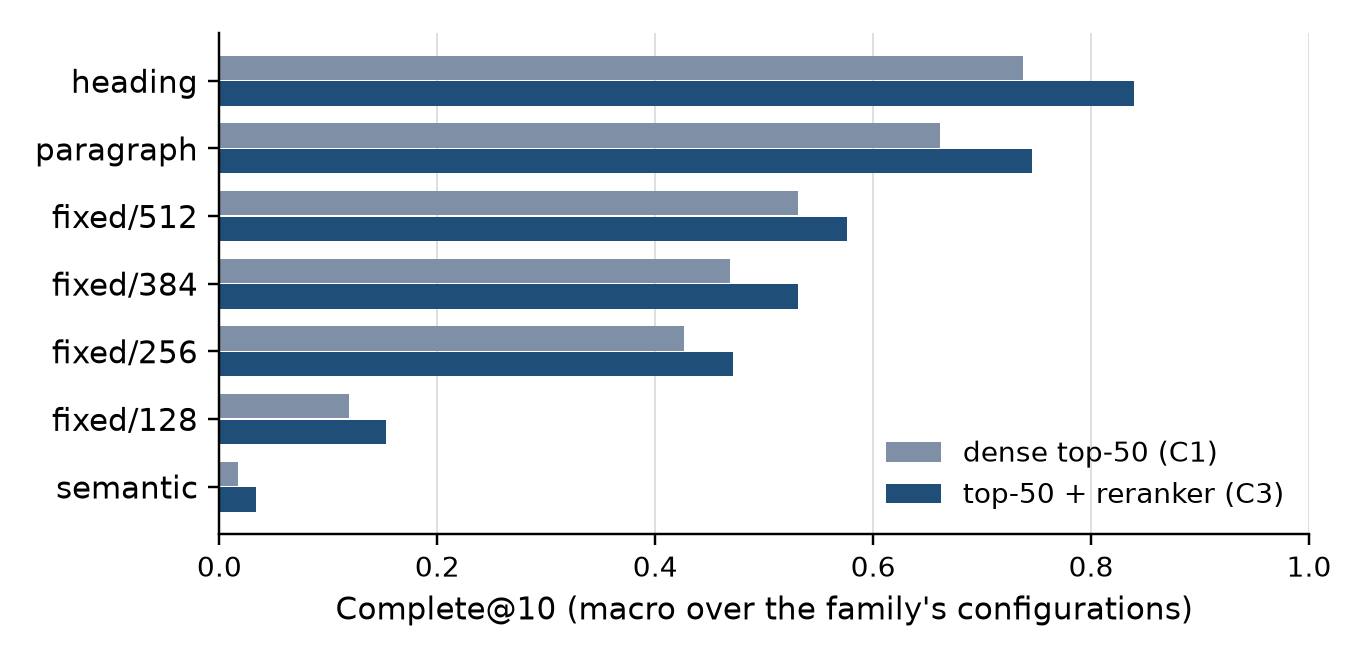
\includegraphics[width=\columnwidth]{figures/family_bars.png}
\caption{Per-family Complete@10 on the first test split, before (C1) and after (C3) reranking. The ordering is stable across tracks; the semantic family is near the floor.}
\label{fig:family}
\end{figure}

Table~\ref{tab:test2} reports the pre-registered supplementary set. The structural-minus-semantic difference on C1 is $+0.800$ [0.666, 0.911]; the observed lower bound, 0.666, exceeded the pre-registered 0.30 threshold. C3$-$C1 is $+0.052$ [0.020, 0.089], a positive direction whose magnitude is not resolved at 45 groups. Because all test2 questions are single-clause, this result concerns complete single-clause evidence, not multi-clause completeness. The positive estimate is evidence for this question composition, not a general confirmation that reranking improves retrieval across question types: test2 is integrity-heavy and was run under a different hardware and run history.

\begin{table}[t]
\centering
\caption{test2: 45 single-clause questions in 45 groups, evaluated once. MRR uses each track's candidate depth (10 or 50).}
\label{tab:test2}
\small
\begin{tabular}{lcc}
\toprule
track & Complete@10 [95\% CI] & MRR\\
\midrule
main & 0.490 [0.422, 0.557] & 0.283\\
C1 & 0.490 [0.422, 0.557] & 0.285\\
C2 & 0.490 [0.422, 0.557] & 0.359\\
C3 & \textbf{0.542} [0.481, 0.601] & \textbf{0.377}\\
\midrule
\multicolumn{3}{l}{structural $-$ semantic (C1): $+0.800$ [0.666, 0.911]}\\
\multicolumn{3}{l}{C3 $-$ C1: $+0.052$ [0.020, 0.089]}\\
\bottomrule
\end{tabular}
\end{table}

\textbf{Candidate pool versus reranking.}
The four tracks separate two changes. C3$-$C1 holds the top-50 pool fixed and applies the reranker, so it isolates reranking within that pool; C3$-$C2 keeps reranking on and expands the pool from 10 to 50. C1$-$main isolates pool expansion without reranking, and C2$-$main isolates reranking at top-10; both are set-level identities because the first ten items are the same set, and the implementation asserts them rather than testing them. C3$-$C1 and C3$-$C2 both equal +0.047 because C1 and C2 have identical Complete@10, but this equality does not attribute the joint gain to one factor: the observed top-10 set requires the combined C3 condition; the available contrasts do not identify separate causal contributions of the two factors.

\textbf{Fixed windows and overlap.}
Within the fixed family, 512-token windows are consistently the strongest setting, and the smallest windows are the weakest. Increasing overlap from 0 to 64 did not monotonically improve completeness. Overlap changes boundary placement and increases redundant text; its net effect depends on whether complete evidence enters the retrieved set. Redundancy competing for top-$k$ slots is a possible explanation, not an established mechanism. The family result should therefore be read as a range of fixed-window behaviours, not as a single tuned baseline.

\textbf{Per-family pattern.}
Figure~\ref{fig:family} shows that the aggregate ordering is not driven by a single configuration. Heading is the strongest family at both tracks (0.737 to 0.839), paragraph is second (0.661 to 0.746), and the best fixed family (512-token windows) reaches 0.531 to 0.576. The two smallest fixed settings degrade sharply, and semantic chunking is close to the floor at both tracks (0.017 to 0.034). The ordering is therefore consistent across granularities, while the gap between heading and paragraph is smaller than the gap between either structural family and the best fixed family.

\textbf{Matched token budget.}
Fixed top-$k$ exposes more text for larger chunks, so we also admit complete chunks in rank order until the next chunk would exceed a token budget, stopping without truncation or skipping. The budget sums each chunk's token count, so overlapping windows are charged repeatedly for their shared text; the budget metrics score the complete admitted chunks, not the tail-truncated text seen by the reranker. Table~\ref{tab:budget} reports recall and Complete@budget at 512, 1024 and 2048 tokens on the test split (C1). Heading and paragraph remain strongest at every budget, while semantic chunking stays near the floor and fixed windows improve with budget but do not close the gap.

\begin{table}[t]
\centering
\caption{Matched token budget, test split, C1: recall/Complete@budget, macro over configurations within each family. Chunks are admitted in rank order until the next would exceed the budget.}
\label{tab:budget}
\small
\begin{tabular}{lccc}
\toprule
family & 512 & 1024 & 2048\\
\midrule
heading & 0.483/0.417 & 0.542/0.483 & 0.642/0.617\\
paragraph & 0.450/0.383 & 0.550/0.500 & 0.650/0.633\\
fixed/512 & 0.278/0.222 & 0.367/0.294 & 0.436/0.367\\
fixed/384 & 0.231/0.194 & 0.311/0.272 & 0.406/0.361\\
fixed/256 & 0.261/0.228 & 0.339/0.289 & 0.469/0.417\\
fixed/128 & 0.086/0.061 & 0.158/0.111 & 0.222/0.161\\
semantic & 0.053/0.011 & 0.072/0.017 & 0.094/0.028\\
\bottomrule
\end{tabular}
\end{table}

\begin{table}[t]
\centering
\caption{Concrete retrieval cases (C1, test split, top-10). Diagnostic replay of the frozen indexes; Hit@10, Complete@10 and Recall@10 match the official C1 per-question records.}
\label{tab:cases}
\small
\resizebox{\columnwidth}{!}{%
\begin{tabular}{llccc}
\toprule
qid & configuration & required & retrieved (rank) & Hit/Comp\\
\midrule
Q0001 & semantic thr0.70 & c8 + c6 & c6 (4); c8 missing & 1 / 0\\
Q0001 & heading & c8 + c6 & c8 + c6 (1) & 1 / 1\\
Q0088 & fixed/128 & 15.053 + c2 & c2 (1); 15.053 missing & 1 / 0\\
Q0088 & heading & 15.053 + c2 & c2 (1), 15.053 (3) & 1 / 1\\
\bottomrule
\end{tabular}}
\end{table}

\textbf{Concrete retrieval cases.}
Table~\ref{tab:cases} reports two post-hoc cases from a diagnostic replay of the frozen indexes
(the replay uses the same C1 retrieval; its per-question values match the official result files).
Q0001 requires clauses c8 and c6: semantic thr0.70 retrieves c6 at rank 4 but no top-10 chunk fully
covers c8, so Hit@10 is 1 and Complete@10 is 0 (recall 0.5); heading retrieves a single chunk at
rank 1 that covers both. Q0088 requires 15.053 and c2: fixed/128 retrieves c2 at rank 1 but not
15.053, while heading retrieves c2 at rank 1 and 15.053 at rank 3. The cases are illustrative, not
a random sample; both show a completeness failure produced by different boundary decisions.

\section{Analysis and Discussion}
\textbf{Boundary fragmentation and incomplete evidence retrieval.}
A union audit on the test split (track C1) shows that 19.5\% of Complete@10-successful question--configuration cells require more than one chunk (71 of 364); for fixed/128 the share is 76.2\%, while heading and paragraph require union in 0\% of their successful cells. These are pooled cell counts within each family, not a macro average of per-configuration shares. The audit associates fragmentation with completeness failures and is indirect evidence about the mechanism; chunk length, truncation, candidate-pool coverage and ranking quality are plausible additional factors.

\textbf{Why semantic chunking is weaker.}
The semantic family is below both structural families at every tested threshold and every matched budget. This is consistent with three non-exclusive mechanisms: sentence-level boundaries can cut a long policy clause; cosine similarity captures topical similarity, not the functional relation between a rule and its exception; and shorter units require several chunks to co-occur in top-$k$, which becomes less likely as the pool fills with near-duplicate fragments. The union audit and the two cases below are consistent with boundary fragmentation, but they do not establish it as the only cause.

\textbf{Clause length.}
Splitting the test questions at the clause-length median gives a short-versus-long difference of $+0.276$ [$-0.019,+0.572$] (Welch interval), which is not statistically resolvable at this sample size; this is not evidence that length has no effect.

\textbf{Reranking.}
On the first test split, the C3$-$C1 gain is small and not significant. On test2 it is positive, but the two sets differ in questions, hardware and code version, so we do not test or imply a between-split difference. The chunking ranking is highly similar before and after reranking (Spearman $\rho=0.963$), which indicates stability of the ordering rather than invariance.

\textbf{Efficiency.}
On the RTX 3060, exact inner-product search had a measured latency of 0.0--3.1 ms per query. Evaluating C3 on the 60-question test split took 12.7--39.2 s per configuration (0.21--0.65 s per query); this range includes reranking and metric computation, uses batch 32, and is not a controlled latency benchmark. Exact search remains substantially cheaper in these runs, but the recorded timings do not provide a controlled estimate of the latency ratio.

\textbf{Relation to prior work.}
The direction of our result agrees with the chunking literature that reports benefits from structure-aware or paragraph-level splitting \cite{mazzitelli2025paragraph,khalib2026chunking}, and with the observation that semantic boundaries can be unstable \cite{kiss2025maxmin,moreno2026growing}. It differs in what is measured: prior work typically reports passage relevance or answer quality, whereas here the outcome is whether the union of retrieved intervals covers every annotated clause. That difference matters for policy text, where a highly relevant passage can still omit the exception. The present results do not establish why the reranking gain is limited; candidate relevance and score distributions would require further analysis. We therefore do not attribute the small gain to the exact index.

\textbf{Document-level heterogeneity.}
For the heading configuration, the macro average over documents (0.7319 under C1) is almost identical to the pooled average (0.7333); under C3 the macro average (0.8935) is higher than the pooled value (0.8333). The two weighting schemes therefore produce different results, which indicates document-level heterogeneity. Because the document weighting follows questions per document rather than document length, the direction of the difference does not establish that smaller documents benefit more; a per-document gain analysis would be needed, and no dominance analysis is reported here.

\textbf{Effect size and interpretation.}
All metric values are proportions in $[0,1]$, while differences lie in $[-1,1]$; intervals use the same proportion scale. A difference of 0.800 therefore corresponds to 80.0 percentage points, but the paper keeps proportions in tables and in the abstract to avoid mixing scales. The first-split reranking interval spans zero, so the correct reading is that an effect of the observed size is compatible with the data, not that no effect exists. The test2 interval excludes zero but is wide, and the single-clause composition limits how far it can be generalised.

\textbf{Practical implications and trade-offs.}
In this corpus and implementation, the best-supported default is a heading- or paragraph-based index: in their successful cells the complete evidence could be covered by a single chunk. Fixed windows are a reasonable fallback when structure is unavailable, but small windows depend on retrieving several chunks together and therefore on ranking. The three tested semantic configurations (thresholds 0.70, 0.75 and 0.80) performed poorly under this objective; we do not generalise this to all semantic methods. The recorded evaluation timings suggest a substantially higher reranker cost, but they do not provide a controlled estimate of the latency ratio; the completeness gain is positive on the supplementary set but not resolved on the first test split, and whether that trade-off is acceptable is a deployment decision, not something these experiments settle.

\section{Limitations}
The first test split was used as a pilot before the reranker stage, so its results are exploratory. test2 is single-clause by construction and cannot validate multi-clause evidence completeness; it is also integrity-heavy and Glasgow-heavy relative to the corpus. The test2 questions were drafted by the AI and jointly reviewed by us with the AI after evaluation, so no independent human annotation exists. The study measures retrieval evidence completeness only and does not evaluate answer generation. The live corpus can no longer be rebuilt byte-identically from the web, so retrieval replay relies on the published snapshot and official indexes. The evaluation environment is only partially recorded, and the two official runs used different GPUs and code versions. \textbf{Threats to validity.}
Internal validity is limited by the single corpus and by the fact that the first test split had been exposed before the reranker stage. Construct validity is limited because completeness is defined by annotated spans: a different annotator could draw a boundary slightly differently, and the union rule rewards contiguous coverage but not semantic equivalence. External validity is limited by the English-language, policy-domain sample and by the small number of institutions. Statistical validity is limited by 59 and 45 groups: power for small effects is limited and the reranking magnitude remains imprecisely estimated. The intervals, not the point estimates, should be used for decisions.

The \texttt{resources} domain is thin (seven questions in the first test set), and no confidence interval is reported for it separately.

\textbf{Design implications.}
In this corpus and implementation, the best-supported design is to follow the document's own structure before embedding similarity: heading-based indexing where headings are reliable, paragraph-based splitting as a fallback, and fixed windows large enough to contain a clause when structure is unavailable. The three tested semantic configurations were weak under this objective; we do not generalise this to all semantic methods. A reranker can be added for a modest gain, but its latency cost should be justified by the application.

\section{Conclusion}
We compared 17 chunking configurations for evidence-complete retrieval over course-policy text under a frozen encoder and a shared frozen reranker checkpoint. On this corpus and protocol, the tested structure-aware configurations retrieved complete evidence more often than the tested sentence-level semantic configurations; the reranking gain was smaller and not resolved on the first test split, and positive but magnitude-unresolved on the single-clause supplementary set. Within this corpus and implementation, heading- or paragraph-based splitting gave the strongest evidence; the tested sentence-level semantic configurations were weak, and we do not generalise that finding to all semantic methods. Future work should broaden the domain mix, add independent human annotation, and evaluate whether completeness gains translate into answer quality.

\section*{AI Disclosure}
Generative AI (DeepSeek) assisted with code development, question drafting, evidence-candidate generation, and manuscript editing. Codex additionally assisted with code development. We reviewed all 172 questions in the first set and jointly reviewed the 45 test2 questions with AI assistance; the joint review attestation is in the repository. We verified the reported numbers against the executed experiments and remain responsible for all claims. AI did not independently run experiments or generate unverified results.

\bibliographystyle{IEEEtran}
\bibliography{refs}

\end{document}
